This section will survey some of the most important concurrent models of computation. Before diving into the models, we will first discuss the mathematical semantics\footnote{Nowadays we call these semantics denotational} of computation by Scott.

\begin{figure}[h]
	\centering
   \resizebox{0.95\textwidth}{!}{
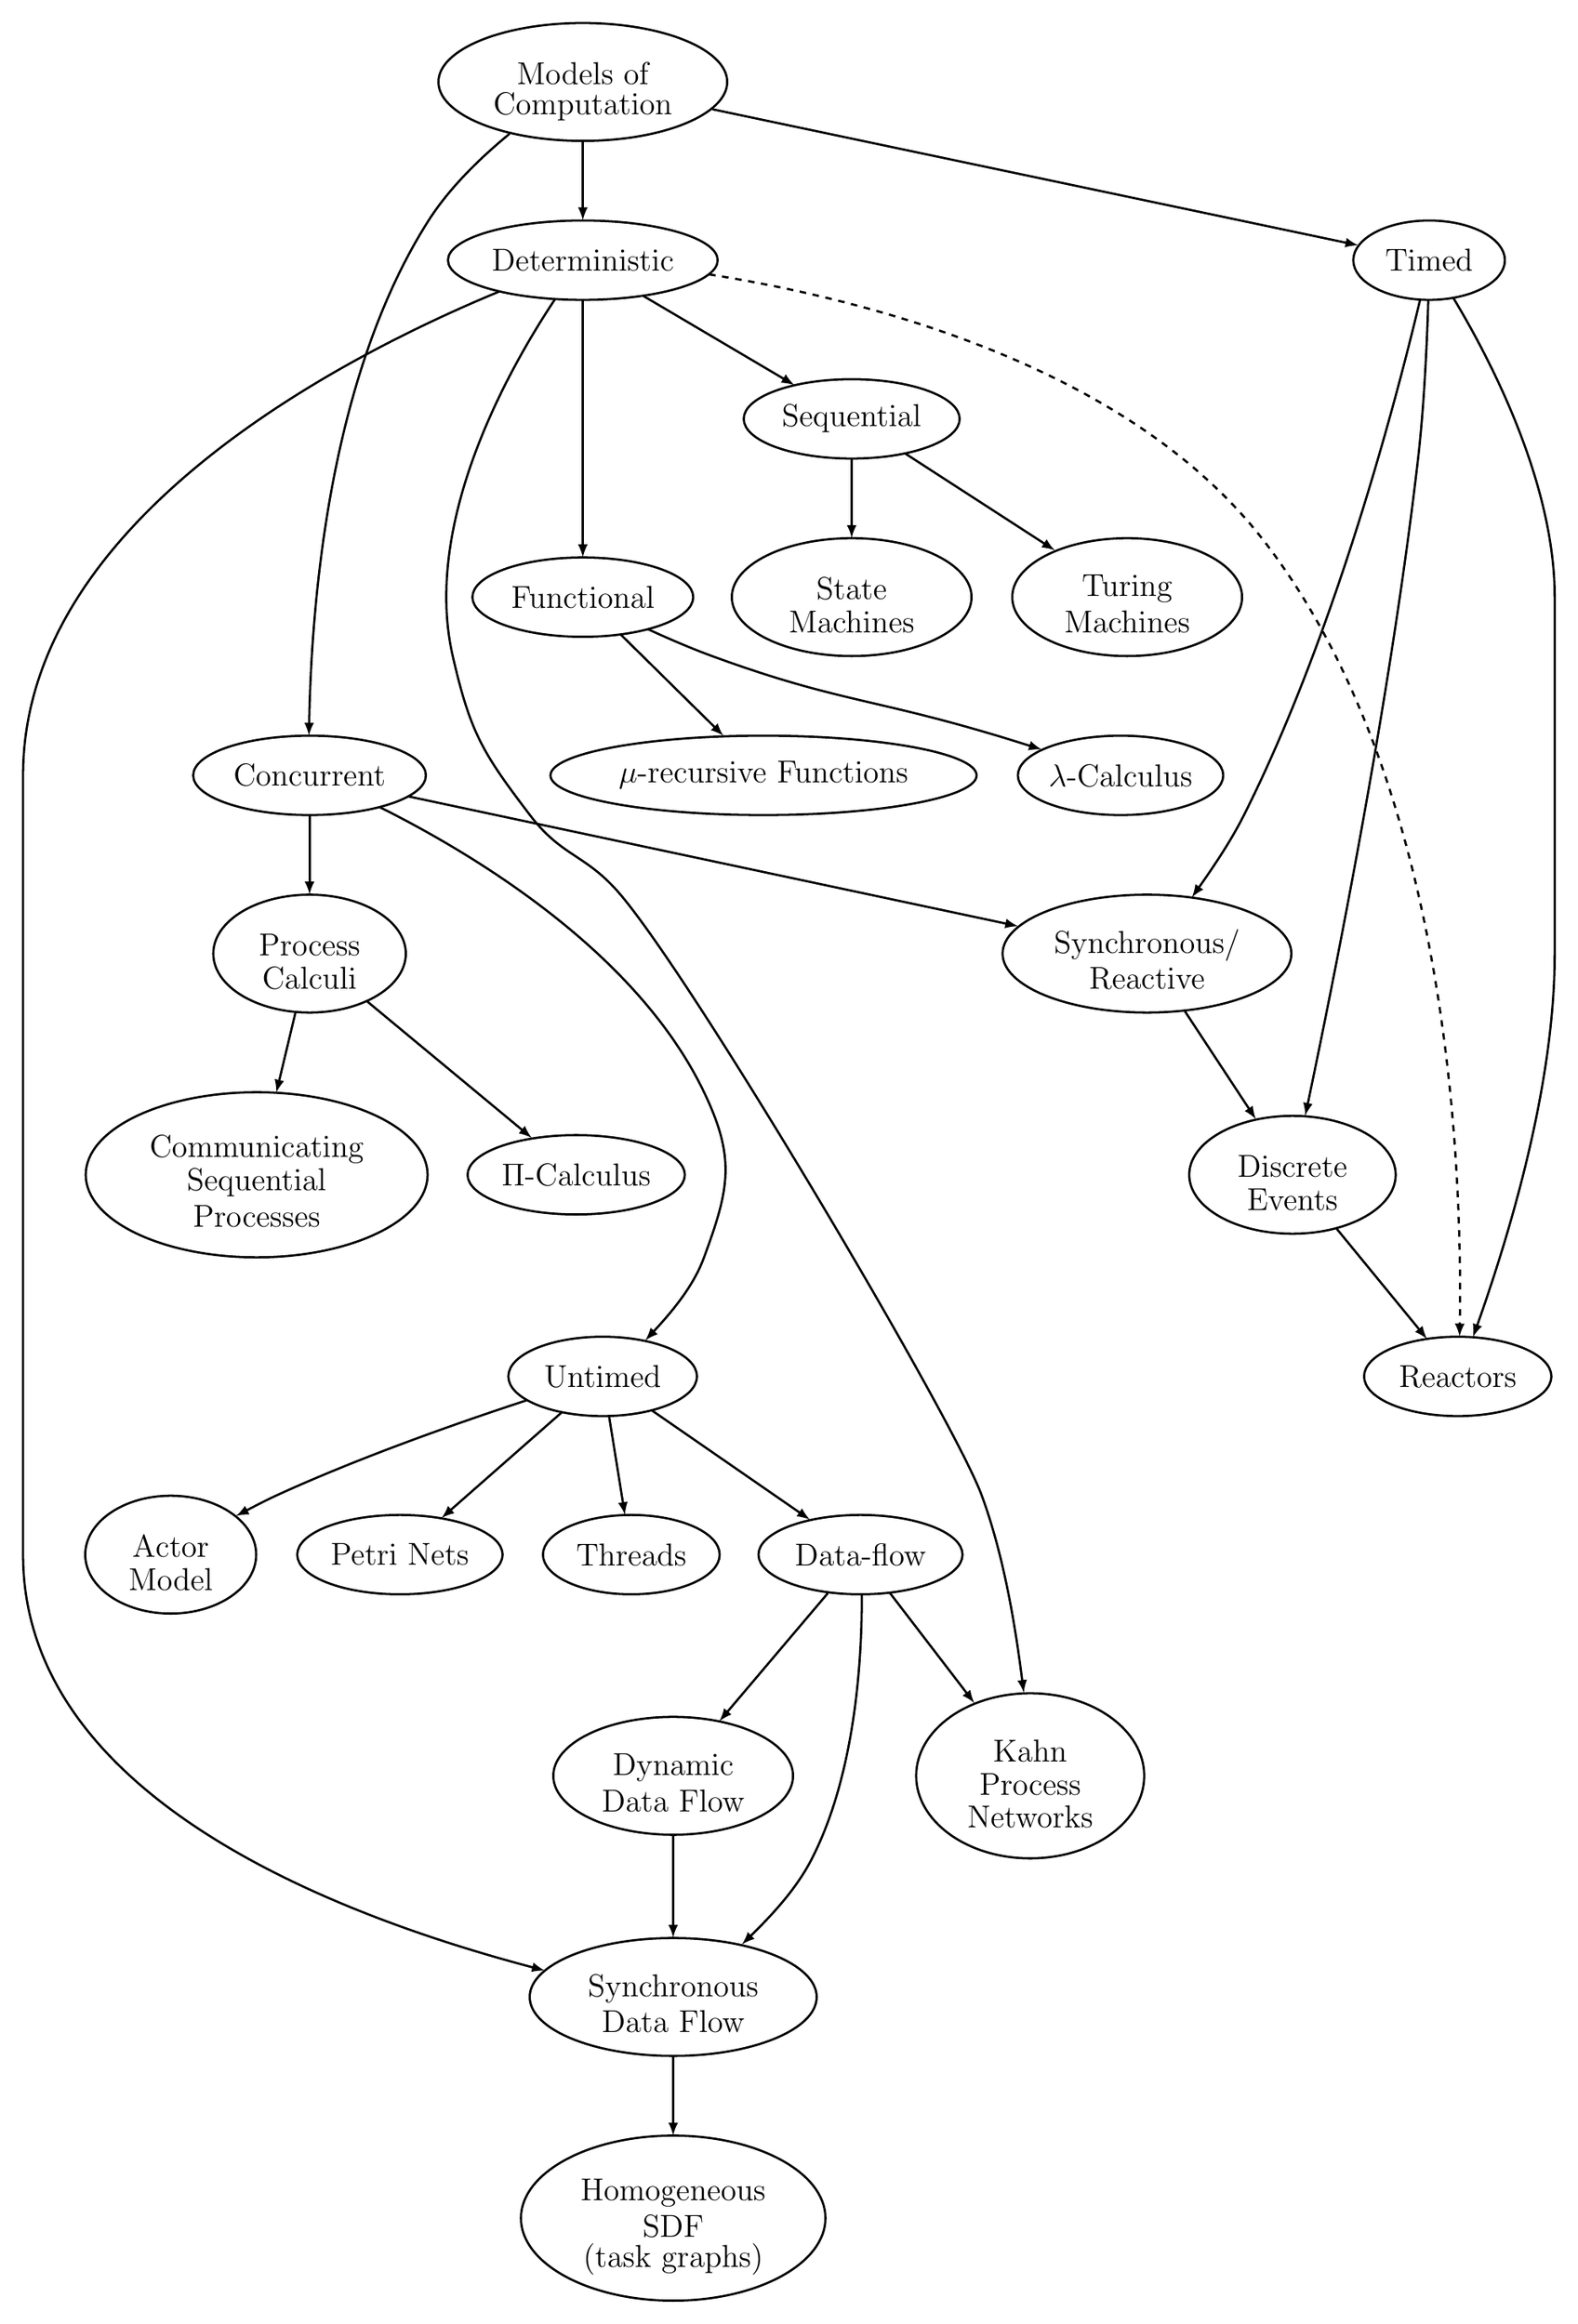
\begin{tikzpicture}[>=latex,line join=bevel,]
  \pgfsetlinewidth{1bp}
\Large%
\pgfsetcolor{black}
  % Edge: root -> concurrent
  \draw [->] (220.74bp,983.16bp) .. controls (207.69bp,972.46bp) and (193.57bp,958.83bp)  .. (184.0bp,943.82bp) .. controls (138.64bp,872.7bp) and (130.81bp,769.62bp)  .. (129.71bp,710.15bp);
  % Edge: root -> t
  \draw [->] (312.74bp,994.32bp) .. controls (390.88bp,977.86bp) and (527.12bp,949.17bp)  .. (605.85bp,932.59bp);
  % Edge: root -> det
  \draw [->] (254.0bp,979.76bp) .. controls (254.0bp,971.49bp) and (254.0bp,962.37bp)  .. (254.0bp,943.97bp);
  % Edge: seq -> touring
  \draw [->] (400.4bp,838.04bp) .. controls (417.23bp,827.14bp) and (440.03bp,812.4bp)  .. (468.15bp,794.2bp);
  % Edge: seq -> sm
  \draw [->] (376.0bp,835.47bp) .. controls (376.0bp,827.9bp) and (376.0bp,818.84bp)  .. (376.0bp,799.82bp);
  % Edge: concurrent -> ut
  \draw [->] (161.9bp,677.64bp) .. controls (204.61bp,656.31bp) and (278.5bp,611.95bp)  .. (309.0bp,548.34bp) .. controls (323.4bp,518.3bp) and (320.51bp,504.65bp)  .. (309.0bp,473.39bp) .. controls (304.9bp,462.24bp) and (297.35bp,451.82bp)  .. (282.39bp,435.75bp);
  % Edge: concurrent -> pc
  \draw [->] (130.0bp,673.73bp) .. controls (130.0bp,666.16bp) and (130.0bp,657.1bp)  .. (130.0bp,638.08bp);
  % Edge: concurrent -> sr
  \draw [->] (174.71bp,682.57bp) .. controls (240.52bp,668.56bp) and (364.01bp,642.28bp)  .. (451.49bp,623.66bp);
  % Edge: t -> sr
  \draw [->] (633.88bp,907.73bp) .. controls (623.81bp,865.35bp) and (595.74bp,757.01bp)  .. (554.0bp,674.08bp) .. controls (549.05bp,664.25bp) and (542.72bp,654.22bp)  .. (530.4bp,636.76bp);
  % Edge: t -> de
  \draw [->] (637.62bp,907.5bp) .. controls (637.08bp,889.27bp) and (635.84bp,860.54bp)  .. (633.0bp,835.82bp) .. controls (620.89bp,730.61bp) and (596.54bp,607.86bp)  .. (581.81bp,537.67bp);
  % Edge: t -> reactors
  \draw [->] (648.99bp,908.71bp) .. controls (665.55bp,881.24bp) and (695.0bp,825.07bp)  .. (695.0bp,772.95bp) .. controls (695.0bp,772.95bp) and (695.0bp,772.95bp)  .. (695.0bp,611.21bp) .. controls (695.0bp,551.4bp) and (674.43bp,483.7bp)  .. (657.97bp,437.32bp);
  % Edge: ut -> petri
  \draw [->] (244.38bp,403.02bp) .. controls (231.0bp,391.26bp) and (212.77bp,375.23bp)  .. (189.91bp,355.14bp);
  % Edge: ut -> df
  \draw [->] (285.28bp,403.99bp) .. controls (303.19bp,391.61bp) and (328.55bp,374.08bp)  .. (357.0bp,354.41bp);
  % Edge: ut -> threads
  \draw [->] (265.95bp,401.04bp) .. controls (267.59bp,390.83bp) and (269.67bp,377.92bp)  .. (273.11bp,356.52bp);
  % Edge: ut -> actors
  \draw [->] (228.58bp,408.57bp) .. controls (198.18bp,398.61bp) and (152.91bp,382.78bp)  .. (115.0bp,365.39bp) .. controls (111.87bp,363.95bp) and (108.66bp,362.38bp)  .. (96.573bp,356.04bp);
  % Edge: det -> seq
  \draw [->] (281.38bp,909.66bp) .. controls (299.09bp,899.21bp) and (322.3bp,885.51bp)  .. (349.97bp,869.18bp);
  % Edge: det -> f
  \draw [->] (254.0bp,907.68bp) .. controls (254.0bp,881.37bp) and (254.0bp,832.34bp)  .. (254.0bp,791.06bp);
  % Edge: det -> sdf
  \draw [->] (215.97bp,911.56bp) .. controls (145.12bp,882.24bp) and (0.0bp,808.04bp)  .. (0.0bp,692.08bp) .. controls (0.0bp,692.08bp) and (0.0bp,692.08bp)  .. (0.0bp,338.52bp) .. controls (0.0bp,229.37bp) and (139.76bp,175.39bp)  .. (236.72bp,149.82bp);
  % Edge: det -> kpn
  \draw [->] (241.3bp,908.01bp) .. controls (220.08bp,876.08bp) and (181.04bp,806.73bp)  .. (195.0bp,746.08bp) .. controls (202.98bp,711.41bp) and (208.43bp,702.38bp)  .. (230.0bp,674.08bp) .. controls (244.7bp,654.8bp) and (255.3bp,656.56bp)  .. (271.0bp,638.08bp) .. controls (305.71bp,597.21bp) and (422.24bp,400.09bp)  .. (435.0bp,365.39bp) .. controls (444.34bp,339.98bp) and (449.76bp,310.24bp)  .. (454.09bp,275.83bp);
  % Edge: det -> reactors
  \draw [->,dashed] (311.3bp,919.38bp) .. controls (382.04bp,908.19bp) and (500.51bp,878.25bp)  .. (562.0bp,799.82bp) .. controls (646.84bp,691.61bp) and (653.12bp,516.23bp)  .. (651.83bp,437.52bp);
  % Edge: f -> mu
  \draw [->] (271.39bp,755.8bp) .. controls (282.79bp,744.56bp) and (297.88bp,729.68bp)  .. (317.78bp,710.05bp);
  % Edge: f -> l
  \draw [->] (283.64bp,758.37bp) .. controls (292.92bp,754.1bp) and (303.27bp,749.63bp)  .. (313.0bp,746.08bp) .. controls (368.92bp,725.68bp) and (384.99bp,727.19bp)  .. (442.0bp,710.08bp) .. controls (445.38bp,709.07bp) and (448.87bp,708.0bp)  .. (462.22bp,703.81bp);
  % Edge: pc -> pic
  \draw [->] (156.26bp,589.44bp) .. controls (175.93bp,573.12bp) and (202.8bp,550.84bp)  .. (230.79bp,527.63bp);
  % Edge: pc -> csp
  \draw [->] (123.63bp,584.58bp) .. controls (121.67bp,576.4bp) and (119.46bp,567.13bp)  .. (114.93bp,548.19bp);
  % Edge: df -> sdf
  \draw [->] (380.58bp,320.47bp) .. controls (380.72bp,293.06bp) and (378.06bp,239.96bp)  .. (358.0bp,200.69bp) .. controls (352.01bp,188.97bp) and (343.03bp,178.08bp)  .. (326.21bp,161.67bp);
  % Edge: df -> ddf
  \draw [->] (365.19bp,321.04bp) .. controls (353.5bp,307.24bp) and (336.86bp,287.59bp)  .. (316.0bp,262.97bp);
  % Edge: df -> kpn
  \draw [->] (393.41bp,321.04bp) .. controls (402.28bp,309.48bp) and (414.3bp,293.82bp)  .. (431.61bp,271.25bp);
  % Edge: sdf -> tg
  \draw [->] (295.0bp,110.93bp) .. controls (295.0bp,103.0bp) and (295.0bp,94.08bp)  .. (295.0bp,75.005bp);
  % Edge: ddf -> sdf
  \draw [->] (295.0bp,211.28bp) .. controls (295.0bp,200.14bp) and (295.0bp,187.04bp)  .. (295.0bp,164.79bp);
  % Edge: sr -> de
  \draw [->] (527.17bp,585.11bp) .. controls (535.31bp,572.72bp) and (545.15bp,557.77bp)  .. (559.37bp,536.14bp);
  % Edge: de -> reactors
  \draw [->] (596.1bp,486.35bp) .. controls (606.71bp,473.41bp) and (619.7bp,457.56bp)  .. (637.02bp,436.44bp);
  % Node: root
\begin{scope}
  \definecolor{strokecol}{rgb}{0.0,0.0,0.0};
  \pgfsetstrokecolor{strokecol}
  \draw (254.0bp,1006.69bp) ellipse (65.52bp and 26.74bp);
  \draw (254.0bp,1010.49bp) node {Models of };
  \draw (254.0bp,995.49bp) node { Computation};
\end{scope}
  % Node: concurrent
\begin{scope}
  \definecolor{strokecol}{rgb}{0.0,0.0,0.0};
  \pgfsetstrokecolor{strokecol}
  \draw (130.0bp,692.08bp) ellipse (52.79bp and 18.0bp);
  \draw (130.0bp,692.08bp) node {Concurrent};
\end{scope}
  % Node: t
\begin{scope}
  \definecolor{strokecol}{rgb}{0.0,0.0,0.0};
  \pgfsetstrokecolor{strokecol}
  \draw (638.0bp,925.82bp) ellipse (34.39bp and 18.0bp);
  \draw (638.0bp,925.82bp) node {Timed};
\end{scope}
  % Node: det
\begin{scope}
  \definecolor{strokecol}{rgb}{0.0,0.0,0.0};
  \pgfsetstrokecolor{strokecol}
  \draw (254.0bp,925.82bp) ellipse (61.19bp and 18.0bp);
  \draw (254.0bp,925.82bp) node {Deterministic};
\end{scope}
  % Node: seq
\begin{scope}
  \definecolor{strokecol}{rgb}{0.0,0.0,0.0};
  \pgfsetstrokecolor{strokecol}
  \draw (376.0bp,853.82bp) ellipse (48.99bp and 18.0bp);
  \draw (376.0bp,853.82bp) node {Sequential};
\end{scope}
  % Node: f
\begin{scope}
  \definecolor{strokecol}{rgb}{0.0,0.0,0.0};
  \pgfsetstrokecolor{strokecol}
  \draw (254.0bp,772.95bp) ellipse (50.09bp and 18.0bp);
  \draw (254.0bp,772.95bp) node {Functional};
\end{scope}
  % Node: touring
\begin{scope}
  \definecolor{strokecol}{rgb}{0.0,0.0,0.0};
  \pgfsetstrokecolor{strokecol}
  \draw (501.0bp,772.95bp) ellipse (52.15bp and 26.74bp);
  \draw (501.0bp,776.75bp) node {Turing };
  \draw (501.0bp,761.75bp) node { Machines};
\end{scope}
  % Node: sm
\begin{scope}
  \definecolor{strokecol}{rgb}{0.0,0.0,0.0};
  \pgfsetstrokecolor{strokecol}
  \draw (376.0bp,772.95bp) ellipse (54.39bp and 26.74bp);
  \draw (376.0bp,776.75bp) node {State };
  \draw (376.0bp,761.75bp) node {  Machines};
\end{scope}
  % Node: ut
\begin{scope}
  \definecolor{strokecol}{rgb}{0.0,0.0,0.0};
  \pgfsetstrokecolor{strokecol}
  \draw (263.0bp,419.39bp) ellipse (42.79bp and 18.0bp);
  \draw (263.0bp,419.39bp) node {Untimed};
\end{scope}
  % Node: pc
\begin{scope}
  \definecolor{strokecol}{rgb}{0.0,0.0,0.0};
  \pgfsetstrokecolor{strokecol}
  \draw (130.0bp,611.21bp) ellipse (43.68bp and 26.74bp);
  \draw (130.0bp,615.01bp) node {Process };
  \draw (130.0bp,600.01bp) node { Calculi};
\end{scope}
  % Node: sr
\begin{scope}
  \definecolor{strokecol}{rgb}{0.0,0.0,0.0};
  \pgfsetstrokecolor{strokecol}
  \draw (510.0bp,611.21bp) ellipse (65.52bp and 26.74bp);
  \draw (510.0bp,615.01bp) node {Synchronous/};
  \draw (510.0bp,600.01bp) node { Reactive};
\end{scope}
  % Node: kpn
\begin{scope}
  \definecolor{strokecol}{rgb}{0.0,0.0,0.0};
  \pgfsetstrokecolor{strokecol}
  \draw (457.0bp,238.17bp) ellipse (51.74bp and 37.45bp);
  \draw (457.0bp,249.47bp) node {Kahn };
  \draw (457.0bp,234.47bp) node { Process };
  \draw (457.0bp,219.47bp) node { Networks};
\end{scope}
  % Node: de
\begin{scope}
  \definecolor{strokecol}{rgb}{0.0,0.0,0.0};
  \pgfsetstrokecolor{strokecol}
  \draw (576.0bp,510.86bp) ellipse (46.84bp and 26.74bp);
  \draw (576.0bp,514.66bp) node {Discrete };
  \draw (576.0bp,499.66bp) node { Events};
\end{scope}
  % Node: reactors
\begin{scope}
  \definecolor{strokecol}{rgb}{0.0,0.0,0.0};
  \pgfsetstrokecolor{strokecol}
  \draw (651.0bp,419.39bp) ellipse (42.49bp and 18.0bp);
  \draw (651.0bp,419.39bp) node {Reactors};
\end{scope}
  % Node: petri
\begin{scope}
  \definecolor{strokecol}{rgb}{0.0,0.0,0.0};
  \pgfsetstrokecolor{strokecol}
  \draw (171.0bp,338.52bp) ellipse (46.59bp and 18.0bp);
  \draw (171.0bp,338.52bp) node {Petri Nets};
\end{scope}
  % Node: df
\begin{scope}
  \definecolor{strokecol}{rgb}{0.0,0.0,0.0};
  \pgfsetstrokecolor{strokecol}
  \draw (380.0bp,338.52bp) ellipse (46.29bp and 18.0bp);
  \draw (380.0bp,338.52bp) node {Data-flow};
\end{scope}
  % Node: threads
\begin{scope}
  \definecolor{strokecol}{rgb}{0.0,0.0,0.0};
  \pgfsetstrokecolor{strokecol}
  \draw (276.0bp,338.52bp) ellipse (40.09bp and 18.0bp);
  \draw (276.0bp,338.52bp) node {Threads};
\end{scope}
  % Node: actors
\begin{scope}
  \definecolor{strokecol}{rgb}{0.0,0.0,0.0};
  \pgfsetstrokecolor{strokecol}
  \draw (67.0bp,338.52bp) ellipse (38.78bp and 26.74bp);
  \draw (67.0bp,342.32bp) node {Actor };
  \draw (67.0bp,327.32bp) node { Model};
\end{scope}
  % Node: sdf
\begin{scope}
  \definecolor{strokecol}{rgb}{0.0,0.0,0.0};
  \pgfsetstrokecolor{strokecol}
  \draw (295.0bp,137.82bp) ellipse (65.11bp and 26.74bp);
  \draw (295.0bp,141.62bp) node {Synchronous };
  \draw (295.0bp,126.62bp) node { Data Flow};
\end{scope}
  % Node: mu
\begin{scope}
  \definecolor{strokecol}{rgb}{0.0,0.0,0.0};
  \pgfsetstrokecolor{strokecol}
  \draw (336.0bp,692.08bp) ellipse (96.68bp and 18.0bp);
  \draw (336.0bp,692.08bp) node {$\mu$-recursive Functions};
\end{scope}
  % Node: l
\begin{scope}
  \definecolor{strokecol}{rgb}{0.0,0.0,0.0};
  \pgfsetstrokecolor{strokecol}
  \draw (498.0bp,692.08bp) ellipse (46.59bp and 18.0bp);
  \draw (498.0bp,692.08bp) node {$\lambda$-Calculus};
\end{scope}
  % Node: pic
\begin{scope}
  \definecolor{strokecol}{rgb}{0.0,0.0,0.0};
  \pgfsetstrokecolor{strokecol}
  \draw (251.0bp,510.86bp) ellipse (49.29bp and 18.0bp);
  \draw (251.0bp,510.86bp) node {$\Pi$-Calculus};
\end{scope}
  % Node: csp
\begin{scope}
  \definecolor{strokecol}{rgb}{0.0,0.0,0.0};
  \pgfsetstrokecolor{strokecol}
  \draw (106.0bp,510.86bp) ellipse (77.56bp and 37.45bp);
  \draw (106.0bp,522.16bp) node {Communicating };
  \draw (106.0bp,507.16bp) node { Sequential  };
  \draw (106.0bp,492.16bp) node { Processes};
\end{scope}
  % Node: ddf
\begin{scope}
  \definecolor{strokecol}{rgb}{0.0,0.0,0.0};
  \pgfsetstrokecolor{strokecol}
  \draw (295.0bp,238.17bp) ellipse (54.39bp and 26.74bp);
  \draw (295.0bp,241.97bp) node {Dynamic };
  \draw (295.0bp,226.97bp) node { Data Flow};
\end{scope}
  % Node: tg
\begin{scope}
  \definecolor{strokecol}{rgb}{0.0,0.0,0.0};
  \pgfsetstrokecolor{strokecol}
  \draw (295.0bp,37.48bp) ellipse (69.09bp and 37.45bp);
  \draw (295.0bp,48.78bp) node {Homogeneous };
  \draw (295.0bp,33.78bp) node { SDF };
  \draw (295.0bp,18.78bp) node { (task graphs)};
\end{scope}
%
\end{tikzpicture}
}
	\caption{Overview of different models of computation.}
	\label{fig:dataflow_mocs}
\end{figure}



\subsection{Partial Computation: Scott Domains}

When Dana Scott proposed his mathematical theory of computation~\cite{scott1970}, he used the term mathematical to contrast it with operational computation.
In practice, the steps of a computation are defined by the \ac{ISA} of the machine executing them.
Most people don't write programs directly for the \ac{ISA}, however. They write them in an abstract programming language, which is translated by a compiler into machine instructions.
Thus, in practice, the implementation of a compiler is what defines the (operational) semantics of programs.
Scott's theory had the ambitious goal of being an abstraction that sat between these operational semantics and the abstract notions of computability of e.g. Church or Turing.
He intended to abstract away the arbitrary implementation choices that were necessary but did not change the essence of the execution.
While today his model is not the single established abstract model of semantics he sought out to define, it introduced several important ideas and mathematical structures to models of computation.
In particular, a crucial abstraction introduced by his theory is that of partial computation.
His theory makes it possible to express a computation as a series of partial results, without regarding the actual implementation of these.
We will now introduce the basics of Scott's mathematical theory of computation.

Two related concepts define computation in Scott's formulation, $\omega$-complete partial orders~\cite{gunter} or complete semi-lattices~\cite{lee_matsikoudis_semantics}. \index{$\omega$-complete partial order}
We will use the latter.
Let $\langle A, \leq \rangle$ be a \ac{poset}. For a subset $B \subseteq A$, we say $a$ is an upper or lower bound of $B$ if $a \geq b$ (resp. $\leq$) for all $b \in B$. 
Similarly, we say $a$ is a \emph{greatest lower bound}/\emph{least upper bound} of $B$ if $a$ is a lower/upper bound of $B$ and for all other lower/upper bounds $a'$ we have $a \leq/\geq b$.\index{(greatest) lower bound}\index{(least) upper bound}
A nonempty set $D \subseteq A$ is then called \emph{directed} if every nonempty subset of $D$ has an upper bound \index{directed set}. If every such set $D$ has a least upper bound, we say that $A$ is directed-complete.
If $A$ additionally has a least element $\bot \in A$ with $\bot \leq a$ for all $a \in A$, we say that $A$ is a complete partial order.
If, instead, $A$ is directed-complete and every non-empty subset has a greatest lower bound, we say $A$ is a complete semilattice.\index{complete semilattice}

The canonical example of this are sequences, which are a generalization of strings. Let $\Sigma$ be an alphabet (a set). 
We call $\Sigma^*$ the set of words (Kleene star) over $\Sigma$, and $\Sigma^\omega = \mathbb{N} \rightarrow \Sigma$ is the set of (countably) infinite sequences over $\Sigma$.\index{Kleene star}
We then define $S = \Sigma^* \cup \Sigma^\omega$ as the set of (finite or infinite) sequences over the alphabet $\Sigma$.\index{sequences}
The set of sequences $S$ is obviously a \ac{poset} with the prefix relation $\sqsubseteq$, where $s \sqsubseteq s'$ iff there exists a $t \in S$ with $s.t = s'$.
Here, $(.) : S \rightarrow S$ denotes the concatenation operator (which coincidentally makes $S$ a monoid with neutral element $\epsilon$, the empty string).
In fact, $S$ is a complete semilattice with regards to $\sqsubseteq$ (cf.~\cite{lee_matsikoudis_semantics}).
In Scott's model, these sequences describe the partial steps of a computation, which generate data in discrete steps (not necessarily all at once). 

A function $f : S \rightarrow S$ is called monotone if for $s \sqsubseteq s'$ it holds that $f(s) \sqsubseteq s'$.\index{Scott ! monotone function}
As a model of computation, this means models causality: having more input data cannot change the data that has already been output.
In other words, the future cannot change the past.
A more technical term is continuity.\index{Scott ! continuity}
A monotone function $f : S \rightarrow S$ is called continuous if for all directed sets $D$ in $S$, it holds that $f (\sqcup D) = \sqcup f(D) := \sqcup \{ f(s) \mid s \in D \}$.
This is distinct from monotone only for infinite sequences. It means that a function will not produce its output only after reading an infinite amount of input.
We call this continuous because the prefix relation defines a topology on the set $S$, the Scott topology.\index{Scott ! topology}

\subsection{Concurrent Computation}
Scott's computation model implicitly assumed a sequential computation and Scott-continuous functions are a powerful method for describing partial sequential computations.
Can we also use this model to describe parallel computation?
Gilles Kahn did precisely this, four years after Scott published his mathematical theory of computation. 
He used the formalism of Scott to define a model of parallel computation, based on what he coined as process networks, now known as \acf{KPN}\cite{kahn74}.

The basic idea to generalize the Scott theory of computation for concurrent (parallel) execution is simple.
We compose functions in networks of Scott functions, these are the \ac{KPN}.
These composed functions yield a system of equations.
For example, we can compose a Scott continuous function $f$ with itself by applying it to its output.
This yields an equation: $f(s) = f(f(s))$, which is solved by a fixed point of $f$ (i.e. a sequence $s \in S$ with $f(s)= s$).
A series of related results on such systems of equations and fixed-points by Tarski, Kleene show that such a system always has a least fixed point.
This defines the semantics of \ac{KPN}.
For example, for the case of the single function $f$ as above, if $f$ is the identity function, this least fixed point is $\epsilon$.
This solves problems with loops in the system by giving well-defined semantics, and even yields a procedure to find the fixed points, by recursively applying the functions.
In particular, this means that \ac{KPN} are deterministic (as per their fixed-point semantics).

There are other related models that span from the same time period, like the Hewitt-Agha actor model\index{actor model}~\cite{DBLP:conf/ijcai/HewittBS73,Agha:86:Actors}.
This was also a model of parallell computation. In it, actors communicate with other actors via mailboxes in a non-deterministic fashion. 
Actors can also be dynamically created and the connections between them are also dynamic.
While this yields much more flexibility, it comes with a high price: deteriminism. 

Other models of parallel computation include Petri Nets\index{Petri nets}~\cite{petri1962nets}, in which a bipartite graph of places and transitions models the distributed execution of a system.
Transitions in petri nets are very flexible as well, but they are also non-deterministic, the order in which multiple activated transitions fire is non-deterministic in general.

A series of more abstract models are the Process Calculi\index{Process Calculi}, which includes the well-known $\Pi$-calculus\index{Process Calculi ! Pi-Calculus} and \ac{CSP}.\index{Process Calculi ! CSP}
These models are called calculi because they define specific composition rules, like parallel composition $A | B$ or $A \| B$ for processes with clear semantics. 
They are well-known for describing systems and specifying their behavior, e.g. in the context of model checking~\cite{baier_mc}.
Technically, however, these are also very abstract models of computation.

\subsection{Dataflow Models of Computation}

A series of models stands out in the context of software synthesis and also in the domain of embedded system software, these are dataflow models of computation.
Wore dataflow models have been with diverse semantics have been proposed than we could reasonably list here.
The original idea however, or at least one of the first to be published, goes back to Dennis~\cite{dennis1974first,dennis1986data}\index{Dataflow ! Dennis}
These dataflow models were also related with \ac{KPN}, in so-called dataflow process networks~\cite{lee1995dataflow,lee_matsikoudis_semantics}
Common among most dataflow models is the concepts of actors, which encapsulate computation and which have \emph{firing} semantics.\index{firing}
Actors communicate exclusively via explicit input and output channels, which work as \acs{FIFO} buffers.
An actor fires when certain conditions are met, consuming tokens in (some of) its input channels, and producing other tokens in its output channels.

We will describe Dennis dataflow using a formalism similar to the one described in~\cite{Parks:M95/105,lee_matsikoudis_semantics}.
This formalism is very general and allows to describe many other dataflow paradigms as special cases.
The basis of the formalism are the \emph{firirng rules}\index{firing rules}.
An actor has a finite set $\mathcal{R}$ of firing rules, and each rule $R \in \mathcal{R}$ is a finite tuple of word over the alphabet of values $\bar \Sigma := \Sigma \cup {\bot}$.
Here, $\bot$ represents an \emph{abscent} value\index{abscent value}, which means no data has to be present in that channel for the actor to fire.
%In the literature\footnote{}, the formulation it is not clear about whether $\mathcal{R}$ has to be finite, but we will demand it is for simplicity, since we don't see any practical value in the case where it is truly infinite.
The patterns sometimes are also interpreted to be words in an extended alphabet with wildcards, e.g. $\Sigma \cup {\bot,*}$, where $*$ stands for any value.
Note that, mathematically speaking, both $\bot$ and $*$ are unnecessary, as the empty string $\epsilon$ has the same effect as $\bot$ and $*$ can be replaced by a series of rules, one for each value in $\Sigma$.
In most pratical instances of dataflow, on the other hand, rules only consist of values in $\{\bot,*\}$, which is why they are very useful for descriptions.

An actor fires whenever there is enough tokens in the input channels to satisfy a rule.
Here, satisfying a rule specifically means the rule $R$ is a prefix of the channel values $C$, $R \sqsubseteq C$.
If we include special values $\bot$ and $*$, the pattern has to be interpreted, e.g. by transforming it into the mathematically equivalent variants explained above.
In this case, the tokens are consumed from the channels and the actor executes, computing something and potentially producing some outputs, which are not part of the specification in the firing rules.

Note that there is nothing preventing multiple rules to apply simultaneously. For example, an actor with two inputs could have the rules $(*,\bot)$ and $(\bot,*)$, firing as soon as one of the two channels has a token.
If multiple rules apply simultaneously, there is no general order in which the actor fires and consumes the inputs. 
This means that this model is non-deterministic.
We call this very general, dynamic variant of dataflow \ac{DDF} (alternatively, Dennis Data Flow).\index{Dataflow ! Dynamic}

If we add an additional condition, requiring that for two rules $R,R'$ there is no upper bound $S$ (i.e. with $R \sqsubseteq S, R' \sqsubseteq S$), then we can show that the model is deterministic.
We can even relax this condition somewhat and keep determinism. In~\cite{lee_matsikoudis_semantics}, the authors show this by explicitly constructing a Scott-continuous function from actor firings and embedding the model into \ac{KPN}.
They also discuss possible relaxations.
This deterministic variant of (Dennis) Dataflow is sometimes referred to as \ac{DPN}.\index{Dataflow ! Process Networks}

All these models are very expressive, so much so that they do not permit very strong analysis of their behavior.
In contrast, the \ac{SDF} model\index{Dataflow ! SDF}~\cite{lee1987sdf} has a very well-defined behavior and allows much more analysis to be done statically, like scheduling or bounding the sizes of the channels~\cite{Parks:M95/105}
The firing rates in the \ac{SDF} model are fixed. In the formalism, this means the firing rules are always of the form $(*^{n_1},\ldots,*^{n_k})$, where $*^0 = \epsilon \equiv \bot$.
Moreover, the number of tokens \emph{produced} is also fixed statically, which is not part of the formalism of firing explained above. 
An apparently more strict variant of \ac{SDF} is \ac{HSDF}, in which all the rates are $1$. However, these two are equivalently expressive: every \ac{SDF} graph can be unrolled to an equivalent \ac{HSDF} graph.
The semantics of \ac{HSDF} are basically equivalent with the widespread model of \emph{task graphs}\index{task graphs}, which are widespread in the design of embedded systems and \ac{HLS}.


We discuss two additional variants of dataflow which sit semantically between \ac{SDF} and \ac{DDF}. 
The first variant is \ac{CSDF}\index{Dataflow ! CSDF}~\cite{bilsen1996cycle}, in which the static values of \ac{SDF} are replaced with cycles that repeat, allowing for some controlled dynamism while retaining the analysability.
Finally, \ac{SADF}\index{Dataflow ! SADF}~\cite{theelen2006scenario} is a more general model which allows to enable and disable certain paths in the graph, which are otherwise static.

Figure~\ref{fig:dataflow_mocs} shows a Venn diagram of the dataflow models discussed here and their relationship.
Here we draw the distinctions as strict as possible.
For example, we draw \ac{HSDF} as a subset of \ac{SDF} since definitionally it is, even though they have the same semantic expressive power.
In other words, \ac{HSDF} is an \ac{SDF}, and conversely, not every \ac{SDF} is an \ac{HSDF}, and even though there is exists an equivalent (unrolled) \ac{HSDF}, it is just equivalent, not identical.
We also include \ac{KPN} and the \ac{KMQ} blocking-reads semantics since they are commonly discussed as dataflow models as well.
Since the models are fundamentally different, we have depict them in the Venn diagram as what is embeddable semantically.
Note that we depict\ac{DPN} as being included in \ac{KMQ} (which is proven in~\cite{lee_matsikoudis_semantics}), but we do not know if this inclusion is strict, in other words, if there are \ac{KMQ} models which are not expressable as \ac{DPN}.
We will discuss the difference between \ac{KMQ} and \ac{KPN} in Section~\ref{sec:macqueen}, and show that this inclusion is indeed strict.

\begin{figure}[h]
	\centering
   \resizebox{0.55\textwidth}{!}{\begin{tikzpicture}%[fill opacity=0.3]
%circles
\node[ellipse, fill=green!20, minimum width = 9cm,minimum height = 5cm,draw] (ddf) at (0,3) {};
\node[ellipse, fill=green!60, minimum width = 6.2cm,minimum height = 4.5cm,draw] (kpn) at (1,3) {};
\node[ellipse, fill=green!50, minimum width = 5.5cm,minimum height = 4.0cm,draw] (kmq) at (1,2.8) {};
\node[ellipse, fill=green!70, minimum width = 4.8cm,minimum height = 3.5cm,draw] (csdf) at (1,2.6) {};
\node[ellipse, fill=green!30, minimum width = 3cm,minimum height = 3cm,draw] (sdf) at (1.5,2.5) {SDF};
\node[ellipse, fill=green!40, minimum width = 1.0cm,minimum height = 1.0cm,draw] (hsdf) at (1.5,3.4) {HSDF};

%labels
\node (lbl-ddf) at (-3,3) {DDF};
%\node (lbl-sdf) at (0,1.5) {SDF};
%\node (lbl-hsdf) at (0,0) {HSDF};
\node (lbl-kmq) at (1,4.5) {KMQ};
\node (lbl-sadf) at (-0.6,2.5) {CSDF};
\node (lbl-kpn) at (1,5.0) {KPN};
  
\end{tikzpicture}
}
	\caption{Relationships between different dataflow models of computation.}
	\label{fig:dataflow_mocs}
\end{figure}